\def\be{\begin{equation}}
\def\ee{\end{equation}}

\newcommand{\nucl}[3]{ \ensuremath{ \phantom{\ensuremath{^{#1}_{#2}}} \llap{\ensuremath{^{#1}}} \llap{\ensuremath{_{\rule{0pt}{.75em}#2}}} \mbox{#3} } }


Delete this later

AND I'VE NOW ADDED THIS
\documentclass[12pt]{article}
\usepackage{graphicx}
\usepackage{notoccite}
\usepackage{epigraph} % epigraph
\usepackage{float}
\usepackage[hyphens]{url}
\usepackage[square, numbers, comma, sort&compress]{natbib}  % Use the "Natbib" style for the references in the Bibliography
\usepackage{verbatim,listings}  % Needed for the "comment" environment to make LaTeX comments
\usepackage{array}  % Needed for the "comment" environment to make LaTeX comments
\usepackage{vector}  % Allows "\bvec{}" and "\buvec{}" for "blackboard" style bold vectors in maths

% \documentclass[a4paper,12pt]{article}
%\usepackage[a4paper,vmargin={20mm,20mm},hmargin={20mm,20mm}]{geometry}
\usepackage{amsmath,amsfonts,amsthm,color,psfrag,epsf,graphicx}
% \usepackage{pstricks}
\usepackage{enumerate,caption}
%\usepackage[lined,algonl,boxed]{algorithm2e}
\usepackage[ruled,linesnumbered,vlined]{algorithm2e}
\usepackage{float}
% \SpecialCoor
\def\subsum{\mathit{\Sigma}}




\def\ifthesis{\iftrue}
\setcounter{secnumdepth}{2}
\newenvironment{myindentpar}[1]%
{\begin{list}{}%
		{\setlength{\leftmargin}{#1}}%
		\item[]%
	}
	{\end{list}}




\graphicspath{{Figures/}}  % Location of the graphics files (set up for graphics to be in PDF format)
\usepackage{epigraph} % epigraph
%customize: \setlength{\epigraphwidth}{7cm}\setlength{\epigraphrule}{0pt}
%use: \epigraph{text}{reference}

%customize: \setlength{\epigraphwidth}{7cm}\setlength{\epigraphrule}{0pt}
%use: \epigraph{text}{reference}
\begin{document}
	%\bibliographystyle{iopart-num}
	\bibliographystyle{unsrt}
	%\chapter{Particle In cell} % Write in your own chapter title
	%label{Chapter3}
	%\lhead{Chapter 3. \emph{A Chapter}} % Write in your own chapter title to set the page header
	\section{Introduction}
	\subsection{Energy Demand}
	Rising populations and economic growth in Asia and Africa will lead to a  large increase in the global energy demand over the next century. It is projected that there will be a 30$\%$ increase in energy demand by 2040, leading to an increase in consumption of all modern fuels \cite{outlook2016}. The elevated dependence on fossil fuels is problematic. According to the BP Statistical Review of World Energy \cite{BP}, known reserves of oil will be depleted by 2066, natural gas by 2069 and coal by the early 22nd century based on 2015 rates of consumption. Not only are fossil fuel reserves dwindling but their continued use is in direct contradiction to global commitments of reducing $CO_2$ emissions to tackle climate change. Alternative energy sources are required that are both sustainable and low carbon emitters, preferably carbon free. Nuclear fission is a promising solution, producing no $CO_2$ during operation and with a fuel source that will last over 150 years based on known uranium reserves and current reactor requirements \cite{uranium}. Fission is capable of providing base load power but its adoption has been hindered by poor public approval, high construction and decommissioning costs and fear of nuclear proliferation. Renewable energy sources such as wind and solar are capable of generating carbon free electricity but have problems with low energy density and intermittency. They can therefore not be relied upon to supply base load power. To date fission is the only proven technology capable of meeting base load power demands whilst minimising the emissions of greenhouse gases \cite{fission}. An energy source that can reliably provide carbon free electricity without the risks of nuclear proliferation is desired. This has led to an international effort to develop nuclear fusion as an energy source. 
	\subsection{Nuclear Fusion}
	Nuclear fusion is a technology with the potential to meet humanity's energy demands, emitting no $CO_2$ and producing minimal amounts of short lived radioactive waste in the process. Fusion is the process by which two light nuclei combine to form a heavier nucleus and some by-products. At attainable energies of today's machines, the fusion reaction with the highest probability of occurrence is the reaction between deuterium and tritium, producing a neutron and helium ash as shown below: 
	\begin{equation}
	\nucl{2}{1}{D} + \nucl{3}{1}{T} \to \nucl{4}{2}{He} + \nucl{1}{0}{n} +17.6MeV
	\end{equation}
	
	
	The neutron carries the majority of the released energy (14.1 MeV) with the alpha particle carrying the rest. In a fusion power plant the neutron would travel out of the plasma into a blanket that slows and absorbs the neutron, converting it's kinetic energy into heat. This heat would be used to convert water into steam as in a conventional reactor.
	Deuterium and tritium are both isotopes of hydrogen, the former found in abundance on Earth whilst the latter can be bred from lithium. Both naturally occurring isotopes of lithium react with neutrons to form tritium as shown below: 
\begin{equation}
	\nucl{6}{3}{Li} + \nucl{1}{0}{n} \to  \nucl{4}{2}{He} + \nucl{3}{1}{T}  +4.8MeV
\end{equation}
\begin{equation}
	\nucl{7}{3}{Li} + \nucl{1}{0}{n} \to  \nucl{4}{2}{He} + \nucl{3}{1}{T} + \nucl{1}{0}{n} -2.466MeV
\end{equation}
making lithium an ideal candidate for the blanket material.  There are enough supplies of deuterium and lithium to provide energy from fusion for millions of years based on current energy demands \cite{fusion_fuel}. Not only is the fuel abundant but only a few grams of it is required to be in the reactor during operation. In the case of loss of  control of a fusion reaction, the reaction ceases immediately, there is no capability for a runaway chain reaction to take place. Fusion is therefore inherently safe. 
	In order for fusion to occur the fuel must be heated to millions of degrees so that the positively charged nuclei can become close enough to allow the strong nuclear force to overcome the repulsive Coulomb forces. There exist three ways of containing the hot fuel long enough for fusion to occur. The first is gravitational confinement, a process exclusively used in stars, the second is magnetic confinement and the third inertial confinement. In inertial confinement fusion (ICF), a pellet of fuel is compressed, often by a laser, raising the temperature and density of the fuel so that the conditions required for fusion are met. Magnetic confinement fusion (MCF) uses strong magnetic fields to confine the hot fusion fuel long enough for fusion to occur. The research detailed in this thesis is only relevant to MCF and so the rest of the chapter will focus on this branch of fusion.
	
	In MCF, a gas mixture of deuterium-tritium (DT) fuel is heated to millions of degrees at which point it forms a charged state of matter known as a plasma. The nuclei of the gaseous fuel becomes separated from the electrons, leading to a more complex interaction amongst the particles. These interactions will be described later in the chapter. Numerous techniques have been developed to confine fusion plasmas such as tokamaks, stellarators, pinch devices, and mirror devices. Of these the tokamak is the most developed and extensively studied.
	
	\subsection{Tokamaks}
	The word tokamak is an abbreviation of a Russian phrase  that translates to "Toroidal chamber with magnetic coils". The first tokamak was built at the Kurchatov institute in Moscow and began operating in 1958. Out of all of the approaches to fusion, tokamaks currently hold the world record for highest fusion gain (Q $\approx 0.7$ ) which is the ratio of energy generated by the fusion reactor to the power required to maintain the plasma in steady state. This record is held by JET \cite{Q_record}. The worlds largest tokamak, ITER is currently under construction in Saint Paul-lez-Durance, southern France. A huge international project with 35 nations collaborating. It is designed to achieve a net energy gain, producing more energy from fusion than was put in to operate the machine and heat the fuel. If this is achieved it will be a world first. ITER is intended to be a proof of principle device which will pave the way for a commercial demonstration power plant, DEMO.     
	
	%Before the tokamak, linear devices such as the magnetic mirror were used to confine the plasma. This device relied on ... but they leaked at the ends. A tokamak took the linear device but curled it round to connect the ends, preventing end leakeages.
	
	%A linear field was found to not give adequate confinement, drifts. 
	
	In order to confine the plasma, a tokamak uses a helical magnetic field. This is formed from the superposition of a toroidal field and a poloidal field. The toroidal field is created by magnetic coils that surround the toroidal chamber. The poloidal field is created by driving a toroidal current through the plasma. The toroidal current creates a poloidal magnetic field that encircles the plasma. The toroidal current is induced in the plasma by placing a solenoid at the centre of the torus. Ramping the current in the solenoid produces a time-varying magnetic flux. This time varying flux then induces a current in the surrounding plasma. The plasma is the secondary coil in the transformer circuit with the solenoid the primary coil. The induced current aids in both plasma confinement and heating. Ohmic heating raises the temperature of the plasma due to it's resistivity. The helical field produced by this superposition is not enough to confine the plasma for adequate amounts of time. Additional poloidal field coils are required in order to stabilise and shape the plasma. A schematic of the magnetic field of a tokamak is shown in figure \ref{fig:tokamak}.
	
	\begin{figure}[H]
		\centering
		\includegraphics[width=0.8\textwidth]{tokamak}
		\caption{A schematic of a tokamak. Courtesy of the JET image database.}
		\label{fig:tokamak}
	\end{figure} 
	
	
	The charged particles of a fusion plasma are confined to the helical magnetic field lines. In the ideal case of perfect confinement, particles would remain confined to these field lines, encircling the torus without coming into contact with the walls of the tokamak. However, in reality, cross-field transport, driven by collisions, turbulence and particle drifts, causes the plasma to drift outwards towards the walls. Impinging plasma particles can displace atoms in the wall. In order to prevent damage to important vessel components and avoid contamination of the core plasma, the flow of plasma to the surface of the machine must be controlled. Early machines designed part of the first wall to protrude from the surface, deliberately bringing the plasma into contact with a specific part of the wall. This region of the wall was known as the limiter. Although limiter based tokamaks were able to control where the damage to the wall was occurring, they were still hindered by the ease at which impurities from the limiter could enter the bulk plasma. Impurities act to lower the plasma temperature by radiative cooling. A partially ionised impurity ion will radiate away energy as trapped electrons complete energy transitions. Reducing levels of impurities in the core, especially high Z impurities, is crucial to maintaining sufficiently high temperatures for fusion to occur. An alternative to the limiter was sought, which led to the development of the divertor. 
	
	
	
	
	\subsubsection{Divertor Configuration}
	A divertor is a region of the tokamak where the plasma is intentionally brought into contact with the vessel wall in a controlled manner. This is advantageous as it  allows the plasma-surface interaction to occur far away from the core plasma, reducing the probability of impurities reaching the core plasma. A divertor relies upon the creation of an X-point in the plasma, a null point in the poloidal field. This null point is created by running a current below the plasma , in the same direction as the toroidal plasma current. This current also creates a poloidal field which interacts with the plasma poloidal field to create a small region of null field. A schematic for the fields responsible for the X-point are shown in figure \ref{fig:X-point}.    
	\begin{figure}[H]
		\centering
		\includegraphics[width=0.8\textwidth]{seperatrix}
		\caption{Toroidal cross-section of the currents and subsequent magnetic fields leading to the formation of the X-point. Taken from \cite{nick}.}
		\label{fig:X-point}
	\end{figure} 
	
	Particles begin in the core plasma and follow closed magnetic field lines that do not end on a material surface. Cross-field transport drives particles outwards towards the vessel walls. The separatrix defines the boundary between open and closed magnetic field lines. Particles that travel beyond the separatrix now follow open field lines. These field lines end on a material surface. This region of open field lines is called the Scrape-Off-Layer (SOL).  In the case of a diverted tokamak, these field lines will take the particles to the divertor target. The target is a material surface situated on the lower legs of the X-point. The target can be designed to tolerate the high flux of heat and particles from the impinging plasma. As well as constraining the plasma exhaust to a limited region of the machine and reducing impurity build up in the core, the divertor configuration also allows the tokamak plasma to operate in high confinement mode (H-mode). This is a regime of reduced particle transport, allowing the core to obtain a higher plasma pressure \cite{H-mode}.
	
	
	
	
	
	%\subsection{MAST}
	
	\subsection{Diagnostics of the SOL and Divertor} 
	The SOL is the boundary layer between the core plasma and the material surface of the tokamak wall. Early fusion experiments focused on the core plasma, where the fusion reactions take place, with the edge a secondary concern. However, it was soon realised that understanding the physics of the edge plasma was crucial to achieving a sustained fusion reaction \cite{edge_importance}. Particle transport in the SOL governs the levels of impurities reaching the core plasma from the material surface. It also regulates the levels of fusion ashes in the core plasma. This by-product of the fusion reaction must be removed from the core plasma to avoid dilution of the fusion fuel. Another crucial role of the SOL is determining the heat load on to the tokamak walls. At present, no material is capable of surviving the predicted heat and particle loads reaching the wall of DEMO and beyond that, an operational fusion power plant \cite{DEMO_material}. If fusion is to become a commercial success, this problem must be overcome. This challenge is being tackled from two angles. From the material science side, new materials, such as composites are being developed that have properties enabling them to survive the harsh conditions of a fusion reactor. Low activation materials, resistant to erosion and able to tolerate high heat loads are required. Walls that are able to self-heal such as liquid metal walls are also being investigated as a potential solution \cite{DEMO_material}. As well as developing materials that can handle such extreme conditions, alternative divertor configurations are being explored that aim to reduce heat and particle loads on to the divertor surface, thus easing the demands placed upon the materials. The Super-X divertor configuration aims to reduce power loads to the divertor target by extending the length of the divertor legs below the X-point \cite{GEOFF}. This increases the connection length, a measure of the distance between a point upstream where a plasma particle enters the SOL, to a point downstream where the open field line closes on the divertor target. Increasing the time it takes the plasma to reach the divertor is advantageous as it increases the capability of radiative cooling to reduce the plasma temperature before it hits the divertor target. The theoretical prediction of reduced  target power load using the Super-X configuration is backed up by detailed SOLPS simulations \cite{SOLPS}. This configuration will be tested on MAST-Upgrade, which will begin operations in 2018.
	
	The edge region of the tokamak is clearly of importance and the physics of it must be understood. A wide range of edge diagnostics have been developed in order to measure the plasma conditions, including probe diagnostics, optical systems, spectroscopic instruments and bolometers.  Of these, the most frequently employed are Langmuir probes. A Langmuir probe is a small electrode, placed into contact with the plasma, that is biased to a potential by an external circuit. The bias voltage applied to the probe is swept and the current the probe drains from the plasma at each voltage is recorded. These measurements allow the local electron density ($n_e$) and electron temperature ($T_e$) to be determined. Optical diagnostics include Thomson Scattering (TS),  optical cameras and infra-red cameras. TS provides electron temperature and density measurements by using the dipole radiation emitted from the electrons as they move in an oscillating electric field produced by a high power laser sent into the plasma. The scattered light is collected and used to diagnose the plasma. This light is a broadened line centred around the original laser waveform. The width of the broadening gives a measure of the electron temperature and the area under the spectrum gives the electron density. Optical and infra-red cameras are used to track the motion of filaments and dust particles in the plasma, infra-red cameras can also be used to measure the heat flux to the divertor target. Spectroscopic instruments interrogate the radiation leaving the plasma in the visible to x-ray region and provide information on the impurities present in the plasma, as well as ion temperature measurements. Bolometric systems are frequently used to measure the total radiated power from the divertor plasma. Langmuir probe data analysis will be the focus of this thesis. More information about Langmuir probes can be found in Chapter X. 

 
%Probe Diagnostics
%rotating mach probe, gundestrup probe, emiisive probe, tunnel probe , fmp, BPP %http://indico.ictp.it/event/a04318/session/41/contribution/30/material/0/0.pdf
	%U probe %https://www.mff.cuni.cz/veda/konference/wds/proc/pdf11/WDS11_239_f2_Kovarik.pdf

%Spectroscopic Diagnostics

%Bolometric systems situated all around the vacuum vessel furnish information on the spatial distribution of radiated power in the main plasma and divertor region using sparse-data tomography.
%Spectroscopic instruments and neutral particle analyzers are installed to cover the visible to X-ray wavelength range, delivering information on plasma parameters such as impurity species and density, input particle flux, ion temperature, helium density, fuelling ratio, plasma rotation, and current density.


\subsection{Plasma Physics} 
Plasma constitutes the vast majority of matter in the known universe, it is the main component of the stars and fills the interstellar medium between them. It is estimated that around $97 \to 99  \% $ of standard (non-dark) matter exists in the plasma state \cite{chen2015introduction} but plasma is not so abundant on Earth. The reason for this can be seen from the Saha equation which describes approximately the expected fraction of ionisation for a gas in thermal equilibrium at a given temperature T due to ionising collisions \cite{chen2015introduction}: 
\begin{equation}
\frac{n_i}{n_n} \approx 2.4 \, \times \, 10^{21} \frac{T^{3/2}}{n_i} \exp \left[-\frac{\epsilon_i}{k_B T}\right]
\end{equation}
where $n_{i,n}$ is the number density of ions and neutrals, $\epsilon_i$ is the ionisation energy and $k_B$ is Boltzmann's constant. For typical conditions on Earth, nitrogen in the air has a density of roughly $3 \, \times \, 10^{25}\, m^{-3}$, a temperature of $300$ K and an ionisation energy of $14.5$ eV. At these conditions, the approximate fraction of ionised nitrogen atoms is then a negligible amount
\begin{equation}
\frac{n_i}{n_n} \approx 10^{-122}
\end{equation}
In order for fusion to occur, temperatures inside a tokamak must exceed 10 MK. At these high temperatures the fuel is sufficiently ionised to adopt the plasma state. 
The plasma state is defined as a collection of ions, electrons and neutral particles that exhibit collective behaviour due to long range Coulomb forces that act between the charged particles. Despite being composed of charged particles, the plasma as a whole remains approximately neutral. This is true on large scales as the number of electrons present in the plasma is equal to the positive charge of the ions that lost the electrons during ionisation. It is also true on small scales too as any charge imbalances that are brought about by random thermal fluctuations are quickly neutralised by the movement of the electrons. The low mass of the electron means it is able to respond very quickly to any charge imbalances, either moving towards regions of net positive charge or being repelled away from regions of net negative charge. This approximate neutrality is a property of the plasma known as quasineutrality. 


	%ion to electron temperature ratio
\subsubsection{Single Particle Description of a Plasma}
The most fundamental way to describe a plasma is to examine the trajectories of individual plasma particles as they respond to electric and magnetic fields. Charged particles in electromagnetic fields experience a Lorentz force ($F_L$) and hence their motion can be described by
\begin{equation}
m_i \frac{d \bold{v}_i}{dt} \  = \ \bold{F}_L \ = \ q_i (\bold{E} + \bold{v}_i \times \bold{B})
\label{eq:force}
\end{equation}
For the straightforward case with no electric fields present and a magnetic field orientated along the z-axis the motion can be broken into components
\begin{equation}
m \dot{v_x} = q B v_y \ \ \ m \dot{v_y} = - q B v_x \ \ \ m \dot{v_z} = 0
\label{eq:dot}
\end{equation}
The particle streams along the magnetic field with a velocity $ v_{\parallel} $ while the x and y velocity components are coupled together. By taking derivatives of equation \ref{eq:dot} it is possible to decouple the components perpendicular to the magnetic field. 
\begin{equation}
\ddot{v_x}  =   - {\left(\frac{qB}{m}\right)}^2 v_x  \ \ \   =   - \omega_c^2 v_x  
\label{eq:vx}
\end{equation}
where $\omega_c$ is the cyclotron frequency at which the charged particle gyrates around the magnetic field line. Taking real solutions gives
\begin{equation}
\begin{split}
v_x = v_\perp \cos\omega_c t  \\
v_y = v_\perp \sin\omega_c t
\end{split}
\end{equation}
where the equation for $v_y$ is obtained by solving equation \ref{eq:vx} and substituting the solution into equation \ref{eq:dot}. Integrating these equations then gives the trajectory of the particles 

\begin{equation}
\begin{split}
x = x_0 +  \frac{v_\perp}{\omega_c} \sin \omega_c t \\ 
y = y_0 -  \frac{v_\perp}{\omega_c} \cos \omega_c t \\ 
z = z_0 + v_\parallel t \ \ \ \ \ \ \ \ \ 
\end{split}
\end{equation}
The particles travel parallel to the magnetic field lines whilst performing orbital motion around the field with a radius equal to the Larmor radius ($\rho_L$)
where 
\begin{equation}
\rho_L = \frac{v_\perp}{\omega_c} \ \ = \frac{v_\perp m }{q B}
\end{equation}
The ions and electrons orbit around a guiding center, a fixed point $(x_0, y_0, z_0)$ as shown in figure \ref{fig:larmor}. The particles gyrate in a direction such that the generated magnetic field from the particle opposes the applied magnetic field. Hence the ions and electrons orbit the field in different directions due to their opposing charges and at different frequencies due to their relative mass difference, the ions having the larger orbit.

\begin{figure}[H]
		\centering
		\includegraphics[width=0.8\textwidth]{larmor.pdf}
		\caption{A schematic of the motion of a charged particle in the presence of an external magnetic field with no external electric field. The particle free-streams along the magnetic field and gyrates in the x-y plane perpendicular to the field.}
		\label{fig:larmor}
	\end{figure} 
	



The free streaming of particles along the magnetic field lines combined with their Larmor orbits give the particles a helical trajectory. The presence of other external forces such as gravity, an applied electric field or a gradient in the magnetic field can cause the guiding center of the particles to drift. The motion of the particles is then composed of the usual gyration around field lines plus an additional drift term of the guiding center. This can be seen by introducing an electric field along the x-axis perpendicular to the magnetic field. We now have 
\begin{equation}
\begin{split}
\ \ \ \ \ \ \ddot{v_x} = \omega_c \dot{v_y} = - \omega_c^2 v_x \ \ \ \ \ \ \\ 
\ddot{v_y} = - \omega_c \dot{v_x} = - \omega_c^2 \left(\frac{E_x}{B} + v_y \right)
\end{split}
\end{equation}
Solving the second order differential equation for $v_y$ gives 
\begin{equation}
v_y = v_\perp \sin{\omega_c t}  + \frac{E_x}{B}
\end{equation}
The y velocity now consists of two parts, the original Larmor motion of the particle plus an additional drift of it's guiding centre perpendicular to both the applied magnetic field and the electric field acting on the particle. The drift motion of the guiding centre due to an electric field is called an ExB drift. Physically this drift arises as the charged particle is accelerated by the electric field during the upward half of it's orbit, increasing the Larmor radius and de-accelerated during the downward swing of its orbit, reducing the Larmor radius. The continuous expansion and contraction of the particles orbit causes it to drift, this is illustrated in figure \ref{fig:exb}.
 \begin{figure}[H]
		\centering
		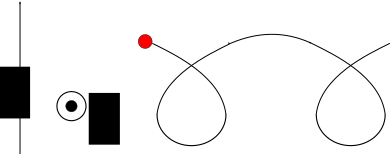
\includegraphics[width=0.8\textwidth]{exb.pdf}
		\caption{The enlargement of the particles orbit as it moves upwards and the contraction as it moves downwards causes the particle to drift in a direction perpendicular to both the electric and magnetic fields.}
		\label{fig:exb}
	\end{figure} 

The drift speed and direction is independent of the particles charge and mass. The ions and electrons orbit the field lines in opposite directions but also gain energy and lose energy from the electric field in opposite directions and so both species drift in the same direction. Therefore there is no net current created by the ExB drift.
%Talk about how the drift speed is indepdent of mass and charge so it is the same for ions and electrons therefore no net current produced. This drift occurs when ever there is a force that acts perpendicular to the magnetic field. Maybe mention the existence of other drifts
	






A complete description of the plasma would be obtained by taking into account the interactions between each particle and every other particle in the system and then by solving equation \ref{eq:force} for every particle. However, it is not feasible to carry out this many calculations on even the most powerful of today’s supercomputers, even for a very sparse plasma. In order to model a plasma, a statistical formulation is required and so the phase space distribution function, $f_{(x,v,t)}$ is introduced. This distribution function represents the probability density of finding a particle with position $x$ and velocity $v$ at time $t$. The evolution of the phase space distribution function for a collision-less plasma is governed by the Vlasov equation 
\begin{equation}
\frac{\partial f}{\partial t}  + \bold{v} \cdot \nabla f + \frac{q}{m} (\bold{E} + \bold{v} \times \bold{B} ) \cdot \nabla_v f = 0
\end{equation}
Solving this equation, or equations derived from it is the principal aim of many codes designed to simulate the behaviour of a plasma in order to test theoretical models and guide experimental work. Numerical solutions to this equation require discretisation techniques to represent the continuous spatial domain of a plasma on a computer. Various approaches to the numerical solution of the Vlasov equation have been developed. These are discussed further in Chapter 3.
%
%	Definition of temperature and the Maxwellian distribution look at Chen intro  
%	Different types of collisions and mean free paths, chaper 3 probably
%	ExB drifts

	
	
	

\subsection{Overview}
Complete this section once other chapters are finalised, 	
\section{References}
\bibliography{references}
\end{document} 

